% Created 2025-05-17 Sat 20:18
% Intended LaTeX compiler: pdflatex
\documentclass{article}


%%%%%%%% ICML 2025 EXAMPLE LATEX SUBMISSION FILE %%%%%%%%%%%%%%%%%
\usepackage[T1]{fontenc}
% Recommended, but optional, packages for figures and better typesetting:
\usepackage{microtype}
\usepackage{graphicx}
\usepackage{subfigure}
\usepackage{booktabs} % for professional tables

% hyperref makes hyperlinks in the resulting PDF.
% If your build breaks (sometimes temporarily if a hyperlink spans a page)
% please comment out the following usepackage line and replace
% \usepackage{icml2025} with \usepackage[nohyperref]{icml2025} above.
\usepackage{hyperref}


% Attempt to make hyperref and algorithmic work together better:
\newcommand{\theHalgorithm}{\arabic{algorithm}}

% Use the following line for the initial blind version submitted for review:
\usepackage[accepted]{style/icml2025}

% If accepted, instead use the following line for the camera-ready submission:
%% \usepackage[accepted]{style/icml2025}

% For theorems and such
\usepackage{amsmath}
\usepackage{amssymb}
\usepackage{mathtools}
\usepackage{amsthm}


% if you use cleveref..
\usepackage[capitalize,noabbrev]{cleveref}
%%%%%%%%%%%%%%%%%%%%%%%%%%%%%%%%
% THEOREMS
%%%%%%%%%%%%%%%%%%%%%%%%%%%%%%%%
\theoremstyle{plain}
\newtheorem{theorem}{Theorem}[section]
\newtheorem{proposition}[theorem]{Proposition}
\newtheorem{lemma}[theorem]{Lemma}
\newtheorem{corollary}[theorem]{Corollary}
\theoremstyle{definition}
\newtheorem{definition}[theorem]{Definition}
\newtheorem{assumption}[theorem]{Assumption}
\theoremstyle{remark}
\newtheorem{remark}[theorem]{Remark}

% Todonotes is useful during development; simply uncomment the next line
%    and comment out the line below the next line to turn off comments
%\usepackage[disable,textsize=tiny]{todonotes}
\usepackage[textsize=tiny]{todonotes}

% The \icmltitle you define below is probably too long as a header.
% Therefore, a short form for the running title is supplied here:
\icmltitlerunning{Test short title ICML 2025}


\usepackage[inkscapelatex=false]{svg}
\date{}
\title{}
\hypersetup{
 pdfauthor={Alan Munoz},
 pdftitle={},
 pdfkeywords={},
 pdfsubject={},
 pdfcreator={Emacs 30.1 (Org mode 9.7.11)}, 
 pdflang={English}}
\usepackage{natbib}
\begin{document}

\twocolumn[
\icmltitle{cp\_measure: Morphological features for bioimaging}

% It is OKAY to include author information, even for blind
% submissions: the style file will automatically remove it for you
% unless you've provided the [accepted] option to the icml2025
% package.

% List of affiliations: The first argument should be a (short)
% identifier you will use later to specify author affiliations
% Academic affiliations should list Department, University, City, Region, Country
% Industry affiliations should list Company, City, Region, Country

% You can specify symbols, otherwise they are numbered in order.
% Ideally, you should not use this facility. Affiliations will be numbered
% in order of appearance and this is the preferred way.
\icmlsetsymbol{equal}{*}

\begin{icmlauthorlist}
\icmlauthor{Al\'an F. Munoz}{broad}
\icmlauthor{Tim Treis}{hh,broad}
\icmlauthor{Alexandr A. Kalinin}{broad}
\icmlauthor{Shatavisha Dasgupta}{broad}
\icmlauthor{Fabian Theis}{hh}
\icmlauthor{Anne E. Carpenter}{broad}
\icmlauthor{Shantanu Singh}{broad}
\end{icmlauthorlist}

\icmlaffiliation{broad}{Broad Institute of MIT and Harvard, United States}
\icmlaffiliation{hh}{Institute of Computational biology, Helmholtz Zentrum München, Germany}

\icmlcorrespondingauthor{Shantanu Singh}{shantanu@broadinstitute.org}

% You may provide any keywords that you
% find helpful for describing your paper; these are used to populate
% the "keywords" metadata in the PDF but will not be shown in the document
\icmlkeywords{Machine Learning, ICML}

\vskip 0.3in
]

% this must go after the closing bracket ] following \twocolumn[ ...

% This command actually creates the footnote in the first column
% listing the affiliations and the copyright notice.
% The command takes one argument, which is text to display at the start of the footnote.
% The \icmlEqualContribution command is standard text for equal contribution.
% Remove it (just {}) if you do not need this facility.

\printAffiliationsAndNotice{}  % leave blank if no need to mention equal contribution
% \printAffiliationsAndNotice{\icmlEqualContribution} % otherwise use the standard text.

\begin{abstract}
Quantifying the contents of objects in images is a common challenge in biological imaging. The most widely used software to do so require significant manual intervention. Here we introduce our library cp\_measure, which provides programmatic access to the most widespread metrics to convert images and objects into features. We then demonstrate that the features are consistent to the standard ones and showcase tasks for which our tool is more suitable than the alternatives. Our tool opens the door to community-driven  development and expansion of bioimage analysis metrics and pipelines, increasing developer accessibility and reproducibility of the pipelines.
\end{abstract}
\section{Introduction}
\label{sec:org4c9ba67}
The field of biological imaging leverages data from cell microscopy images to obtain biological insights. Microscopy techniques allows us to acquire information from a multitude of sources, such as illumination, fluorescent dyes or even proteins tagged with other proteins that fluoresce, acting as a beacon and providing information on quantity and/or localization.

The main task at the core bioimage analysis is identifying features that convey information of the state of a cell or its contents. This entails combining identified objects with pixel data to quantify their morphology and other information sources, such as intensity distributions.

Morphological profiling a subfield of bioimaging that focuses on the cells and the shapes and properties of their organelles. It is usually supported by both statistical methods and machine and deep learning approaches. One of its biggest applications is drug discovery, where it is used primarily due to its low acquisition cost and capabilities for scaling to screen many compounds efficiently \citep{sealDecadeSystematicReview2024}. It can also complement to other high throughput methods, such as genomic sequencing.
\subsection{The current state of bioimage analysis}
\label{sec:org8f5b33d}
The most widely used software to process biological imaging data is CellProfiler \citep{stirlingCellProfiler4Improvements2021}. Its target users are biologists with limited programmatic expertise. While this has been of great benefit for biologists, it has a number of issues that hamper its usability in many contexts.

CellProfiler elicits a higher degree of friction for composite pipelines that orchestrate multiple tools. Its focus on manually-defined workflows adjusted for specific use-cases makes it less suitable for low-customization high throughput analyses, more so since the development of generalist segmentation methods and foundational models. Additionally, its large number of dependencies, which include modules from both the Python and Java, can increase the complexity of setup if one is to integrate CellProfiler with other tools. Tough containerisation mitigates this problem, they are not without their own complexity and caveats.

Though certain morphological features can be obtained using scikit-image, these are a fraction of the current standard and cannot be directly compared to the existing datasets produced using CellProfiler. Another challenge resultant of using CellProfiler is its dependency on human interaction at multiple points, which provides the ability of inspecting and parameterizing data but opens the door to human mistakes and hindering reproducibility.

A CellProfiler pipeline struggles integrating well with other computational tools. Its existing plug-in system is inaccessible for most users and has strong limitations. Building automated pipelines that contain CellProfiler and integrating tools within its components are time and effort-consuming challenges that require a decent understanding of its interfaces. Treating it as a black box is an option, but its adding functionality, such as adding a custom-made image filter is not possible.

There is the need for a software library that covers the generalist and high throughput use-cases for which CellProfiler is inadequate. Distributed CellProfiler would cover this case if not for its cloud-only approach and dependency on preconfigured pipelines, as well as its limited debugging capabilities \citep{mcquinCellProfiler30Nextgeneration2018}. Some tools, such as ScaleFex \citep{comoletHighlyEfficientScalable2024}, attempt to fill this gaping hole in the biological software, but they have limitations: First, their features have completely independent implementations from the original ones, thus are not reproduce existing results and the biological interpretations may be different from the current field standard. Additionally, their implementations are usually an off-the-shelf solution, which works well if they match our use-case, but they are not modular nor usually scale well upon increases to the data size. Other alternatives are directed at cloud-first and neglect the use-cases for which local compute would suffice.
\subsection{Engineered features in the era of deep learning}
\label{sec:org9dc3dfa}
The unprecedented evolution of deep learning methods in recent years has made available many different ways to process imaging data. Nevertheless, these are limited in their capacity to provide biological interpretation \citep{moenDeepLearningCellular2019}. Engineered features can also outperform deep learning ones under certain conditions \citep{tangMorphologicalProfilingDrug2024}. Even as deep learning features improve over time, they still require complex interpretability methods, in the rare case where they can be interpreted. Deep Learning also has a higher barrier of entry, since most models require annotating data for training and testing. The foundational models whose goal is to bypass this step do not generalize well for out-of-distribution data. Unlike deep learning-based features, whose interpretation requires complex methods such as counterfactuals or attention maps, most of the engineered features have a mathematical definition that is vastly simpler to translate into biological insights.

The core target users of such a tool would be biologists and data scientists who need reproducibility and data within a few lines of code. As a whole, there is still a role to be played for engineered features to, at the very least, complement deep learning ones. The community is missing a generalist tool that converts images and masks into representative vectors without the need of interfaces or cloud compute and that integrates seamlessly with other scientific libraries. This is the role that we envision cp\_measure can occupy in the scientific software ecosystem.
\section{Extraction of interpretable features using cp\_measure}
\label{sec:org5633614}
In cp\_measure, we isolated the CellProfiler measurements and categorize them based on their inputs: One object and one imaging channel (e.g., intensity, texture), one object and multiple channels (such as correlation features) and multiple objects (e.g., number of neighbors).

\begin{figure}[htbp]
\centering
\includesvg[width=.9\linewidth]{./figs/cpmeasure_overview}
\caption{\label{fig:overview}Our tool produces features from images by using the local information in every region of interest. This can be used to featurize the pairwise combination of all the available channels. The resultant matrices represent the entirety of the experiment in a much more compressed way, and can be processed with standard machine and deep learning methods.}
\end{figure}

The cp\_measure features were based off the CellProfiler implementation, but we separated the actual functional components (i.e., math) from the user-facing and orchestration components. It improves reusability, testability and its makes it possible for more people to access and improve its internals in the future. We positioned it to become a stepping stone in extensibility and maintainability. By isolating and cleaning the implemented mathematics of CellProfiler we vastly reduce the amount of time and manual effort required to perform data analyses while retaining the features present in numerous datasets.

Our aim is to remain consistent with the current scientific python ecosystem. Its interface corresponds that of the widely used scikit-image \citep{waltScikitimageImageProcessing2014}. This greatly reduces the effort needed to integrate it in existing workflows and tools.

We will now demonstrate the validity and capabilities of cp\_measure in cases that would normally require domain expertise and a considerable amount of time. First, we validate cp\_measure features versus CellProfiler results with a subset of the JUMP dataset \citep{chandrasekaranJUMPCellPainting2023}. Then we showcase cases in which cp\_measure is a more practical choice to process microscopy data: First 3D images of astrocytes and then spatial transcriptomics. These use-cases demonstrate its widespread suitability for different types of problems. 
\subsection{Recapitulating CellProfiler measurements}
\label{sec:org09b0cd2}

\begin{figure}[htbp]
\centering
\includesvg[width=.9\linewidth]{./figs/jump_r2_examples}
\caption{\label{fig:cp_vs_cpmeasure}cp\_measure features match their CellProfiler analogs. \textbf{Left panel.} Representative examples comparing Cellprofiler feature values to cp\_measure's, generated using matching pairs of masks and images. \textbf{Right panel.} \(R^2\) value of a linear fit for each individual feature, comparing cp\_measure to CellProfiler.}
\end{figure}

We first performed the numerical validation of cp\_measure, relative to the original CellProfiler features. In preparation, we collected 300 images corresponding to 150 perturbations from the JUMP dataset. the most significant phenotypes for a given measurement each. To ensure that we are using identical object masks, we segmented these images to obtain the cells and nuclei using CellProfiler, providing object masks and their associated features. Next, we applied cp\_measure on these masks with the original images and mapped the features from cp\_measure to CelProfiler. Lastly, we calculated a linear fit for the matched features and calculated their \(R^2\) value.

The validity of cp\_measure is shown on Figure \ref{fig:cp_vs_cpmeasure}. We show examples of the features on the panel on the left. Mostly straight lines demonstrate the recapitulation of measurements from our implementation. A few data points fall outside the diagonals, which may indicate that some edge-cases are treated differently. The panel on the right shows the \(R^2\) value of a linear interpolation. Given that this value is directly correlated to the correctness of the implementation, we can see that most of our measurements resulted in a linear relation, regardless of whether the masks were for nuclei or cytosols. This result provides reassurance that cp\_measure can be confidently in cases where CellProfiler would be used.
\subsection{Results}
\label{sec:orge5b5c6b}
We showcase a couple of use-cases in which cp\_measure makes our machine-learning workflows faster and integrate better with existing tools.
\subsubsection{Astrocytes 3D data}
\label{sec:org447090b}

As a demonstration of its ease of use and the value of interpretable features, we used cp\_measure in a standard classification workflow. We processed 433 3D images of astrocytes containing 831 cells \citep{kalinin3DCellNuclear2018}. We preprocessed the data following standard procedures \citep{caicedoDataanalysisStrategiesImagebased2017}. Then, we trained a Gradient Boosting classifier to identify the day in which the image of any given cell was acquired. With this we identified which features distinguish cells on the later samples and distinguish subpopulations. Finally, we calculated the Shapley values to get a better understanding of the effects of the drugs on the cells [CITE Shapley].

\begin{figure}[htbp]
\centering
\includesvg[width=.9\linewidth]{./figs/example_shap}
\caption{\label{fig:astrocytes}\textbf{Top panel.} Example pair of astroctyes image and masks. The 3D images were projected over the z-axis, taking the maximum value across the z-stack. \textbf{Bottom panel.} Shapley values of the most important features to classify the day in which an image was taken (out of three). The test data accuracy is shown in bold.}
\end{figure}

Figure \ref{fig:astrocytes} shows an example image and object masks alongside the Shapley values of a classifier trained on cp\_measure features. Our results showcased the axis length of the cell to be a major indicator of phenotypic effect, implying that cells became more elongated on their minor axis. While it was posisble to CellProfiler for this task, cp\_measure made it much faster and simpler to implement, specially since the segmentation masks were already provided, which is quite common in public datasets.
\subsubsection{Spatial transcriptomics}
\label{sec:org5711d86}
A key advantage of providing these measurements as a standalone Python package is their ease of integration into diverse analytical workflows, which otherwise would require substantial adaptation to the standard CellProfiler environment. The recent proliferation of black-box foundation models trained solely on morphological data highlights morphology as a highly informative and predictive modality. However, the feature vectors produced by these models are typically not interpretable, preventing direct biological assessment. In contrast, classical morphological measurements yield explicit, interpretable readouts -- for instance, the co-localization of fluorescent markers -- facilitating clear biological interpretations.

To demonstrate this utility, we integrated our cp\_measure-based feature extraction into the widely used spatial analysis library Squidpy (CITE). Being standalone allowed seamless incorporation into workflows powered by the robust SpatialData (CITE) framework underlying Squidpy. Because spatial datasets often comprise significantly more cells per field-of-view (FOV) than conventional microscopy screenings -- up to approximately 100,000 cells-traditional software typically cannot process these large images without cropping, which introduces boundary artifacts. Leveraging the modular design of cp\_measure, we parallelized feature extraction at the single-cell level, streaming batches of cells across computational cores. This approach enables efficient computation even on large-scale datasets, a feat not achievable with standard CellProfiler software.

To further illustrate the value of morphological features, we evaluated their impact on cell-type prediction tasks using spatial transcriptomics data. This application is particularly compelling, as current spatial transcriptomics technologies typically produce matched histological images that remain largely underutilized beyond visualization. We analyzed two mouse brain datasets generated by Bruker Spatial's CosMx platform (CITE nanostring.com/products/cosmx-spatial-molecular-imager/ffpe-dataset/cosmx-smi-mouse-brain-ffpe-dataset/). Each dataset comprises expression profiles for 960 genes and immunofluorescence images captured via five distinct fluorescent probes ('Histone', 'DNA', 'GFAP', 'G', 'rRNA'). Morphological features were extracted from these 5-channel images for both datasets. Subsequently, both gene expression and morphological data were preprocessed according to best practices established by Scanpy (CITE) and PyCytoMiner (CITE) respectively. We trained an XGBoost model to predict cell types on the larger dataset (48,556 cells; see Fig. XXX, panel XXX), comparing models using either gene expression alone or combined gene expression and morphological data. Model performance was assessed by predicting cell types in a smaller independent dataset (38,996 cells), using the F1-score metric stratified by cell type. Figure XXX (panel XXX) highlights the improved predictive accuracy obtained when morphological features are included. Importantly, this performance enhancement required no additional experimental effort, underscoring the benefit of employing cp\_measure beyond its traditional scope.

\begin{figure}[htbp]
\centering
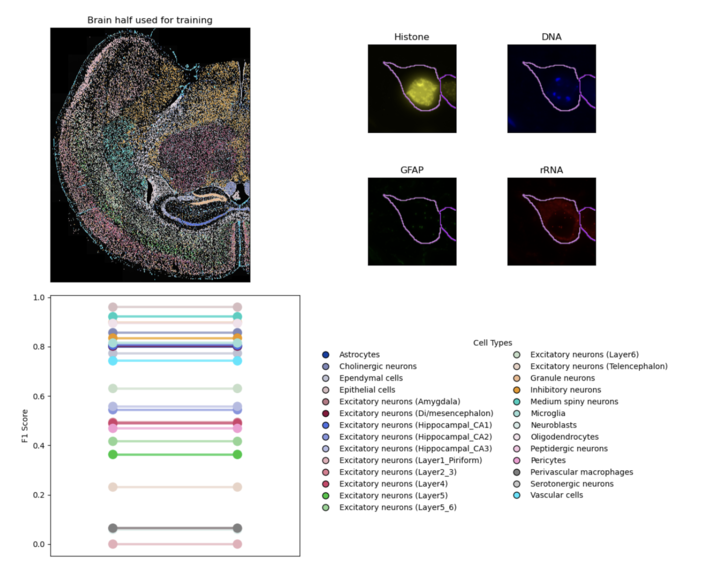
\includegraphics[width=.9\linewidth]{./figs/spatial.png}
\caption{\label{fig:spatial_omics}{[}PLACEHOLDER] Spatial omics analysis.}
\end{figure}
\section{Discussion}
\label{sec:orgf37b369}
The usage of image analysis pipelines that require manual setups hinders reproducibility and hinders our ability to compare different datasets. In this work we introduced our new library cp\_measure, which provides widely used engineered features and enables simpler automated analyses of microscopy data in either short scripts and complex pipelines. This also removes the requirement of using graphical interfaces to process microscopy data, resulting in better scaling capabilities for high-content microscopy even without cloud infrastructure.

The biologically interpretable features provided by cp\_measure complement deep learning ones and offer a better mechanistic understanding of the underlying biology. When used in tandem with generalist tools it enables more insightful pipelines that leverage machine and deep learning approaches. 

These measurements have already been used in non-biological contexts, such as environmental monitoring \citep{ideharaExploringNileRed2025}, thus these engineered metrics also benefit other scientific fields beyond morphological profiling.
\section{Future work}
\label{sec:org5cdbb12}
The most obvious way to make cp\_measure more useful is to contribute it back to CellProfiler. This would ensure that the results from pipelines built with either tool will always be comparable, while also providing the opportunity of formalizing the inputs and outputs of all measurements. 

Developing a comprehensive tests suite will guarantee mathematical correctness, which currently not even CellProfiler has. This test suite in turn would in turn expedite improvements in multiple ways: Firstly, optimizing the most compute-consuming features, such as granularity. Later on, we could add to support just-in-time compiling and GPUs.

Long-term, we envision cp\_measure can be the place to develop and distribute new measurements. While CellProfiler's measurements are already ubiquituous in bioimaging studies, the existing palette of measurements could be further extended to cover unexplored use-cases. We also see adding community-contributed measurements to better match the current questions scientists pose to imaging data.

\bibliographystyle{icml2025}
\bibliography{bibliography}
\end{document}
